\documentclass{report}
\usepackage{graphicx}
\renewcommand{\contentsname}{indice}

%preambolo
\title{\Huge Documentazione ingegneria del software \\[0.5cm]
        \Large Progetto: Webapp per la gestione della glicemia}
\author{Fazion Pietro (VR501347) , Dal Degan Pietro (VR500305)}
\date{}

%inzio del documento
\begin{document}
% pagina 1 (titolo)
\maketitle
\newpage

%pagina 2 (indice)
\tableofcontents

\newpage

%pagina 3 (use case)
\chapter{Azioni degli utenti}

La Webapp che siamo andati a sviluppare è a servizio di tre tipologie di utenti:
\begin{itemize}
    \item Paziente
    \item Medico
    \item Admin
\end{itemize}
Tutte le precedenti categorie di utenti hanno bisogno di autenticarsi per poter
accedere alla propria area riservata.
Andiamo a vedere ora i casi d'uso e i loro diagrammi di sequenza.

\textbf{Per motivi di chiarezza nella visualizzazione delle immagini,\\
 divideremo i casi d'uso per utente, nonostante siano collegati tra loro.}
\\
\section{Casi d'uso del Paziente}
\begin{figure}[h!]
    \centering
    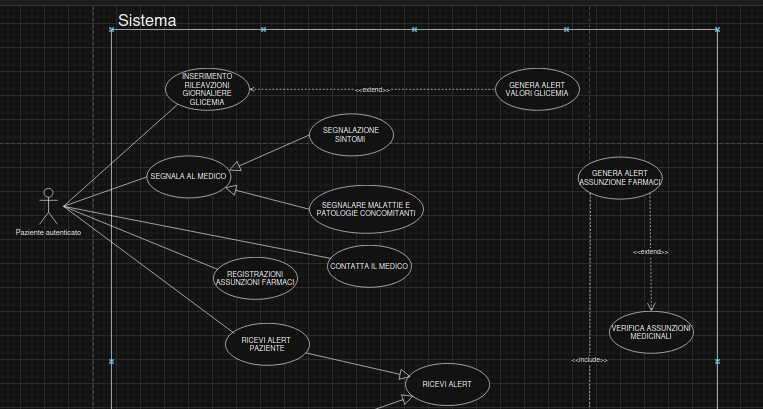
\includegraphics[width=\textwidth, height=0.305\textheight, keepaspectratio]
    {img_relazione/Use_case_paziente.png}
\end{figure}

Dopo esssersi autenticate il paziente verra reindirizzato alla sua homepage,
dove troverà:
\begin{itemize}
    \item Un grafico con l'andamento della sua glicemia nel tempo
    \item Un pulsante per l'inserimento della glicemia
    \item Gli ultimi record di glicemia inseriti
    \item Un form per la comunicazione di sintomi e malattie
    \item Un area per contrassegnare i medicinali assunti
    \item Un form per contattare il medico
\end{itemize}

\vspace{1cm}
Ora elenchiamo di seguito i casi d'uso visti nell'immagine:
\begin{itemize}
    \item Inserimento della rilevazione della glicemia
    \item Segnalazione di patologie, malattie e/o sintomi riscontrati al medico
    \item Registrazione giornaliera di medicinali assunti
    \item Contattare il medico
\end{itemize}
\vspace{0.5cm}
\subsection{inserimento della rilevazione della glicemia}
Il paziente deve essere in grado di poter inserire il livello glicemico,
schiacciando il pulsante "inserisci glicemia" si visualizza un modal dove 
inserire il proprio livello glicemico.

\vspace{0.5cm}

\fbox{
    \begin{minipage}{0.9\textwidth}

        \vspace{0.3cm}
        \textbf{Attori: } Paziente \\
        \textbf{Precondizioni: } Il paziente deve essersi autenticato \\
        \textbf{Passi: } \vspace{0.05cm}
        \begin{enumerate}
            \item Il paziente accede alla sua zona riservata
            \item Il paziente clicca il pulsante "inserisci glicemia"
            \item Il paziente riempie il campo del modal glicemia che compare
            \item Il paziente clicca il pulsante "invia"
            \item Il dato viene salvato nel database
            \item Viene controllata la validità del dato inserito
            \item Eventualmente vengono creati alert per Medico e Paziente in caso
            di valori fuori range
        \end{enumerate}
        \textbf{Postcondizioni: }

    \end{minipage}
}

\begin{figure}[h!]
    \centering
    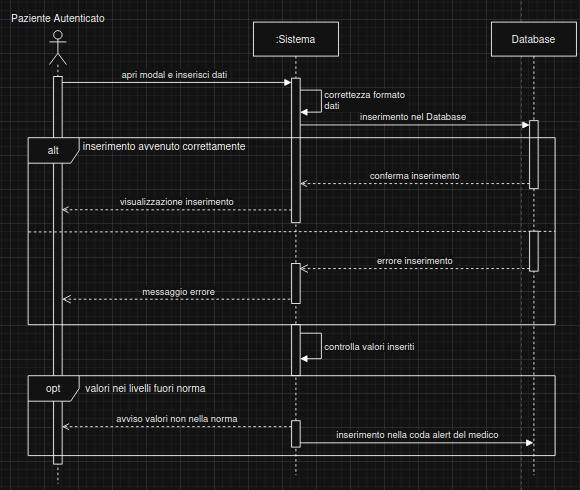
\includegraphics[width=\textwidth, height=\textheight, keepaspectratio]
    {img_relazione/Inserimento_glicemia.png}
\end{figure}



\section{Casi d'uso del Medico}
\begin{figure}[h!]
    \centering
    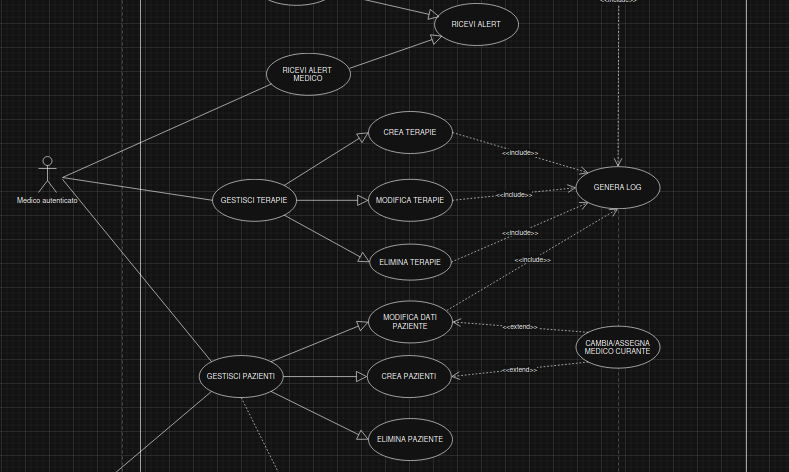
\includegraphics[width=\textwidth, height=\textheight, keepaspectratio]
    {img_relazione/Use_case_medico.png}
\end{figure}

\section{Casi d'uso dell'Admin}
\begin{figure}[h!]
    \centering
    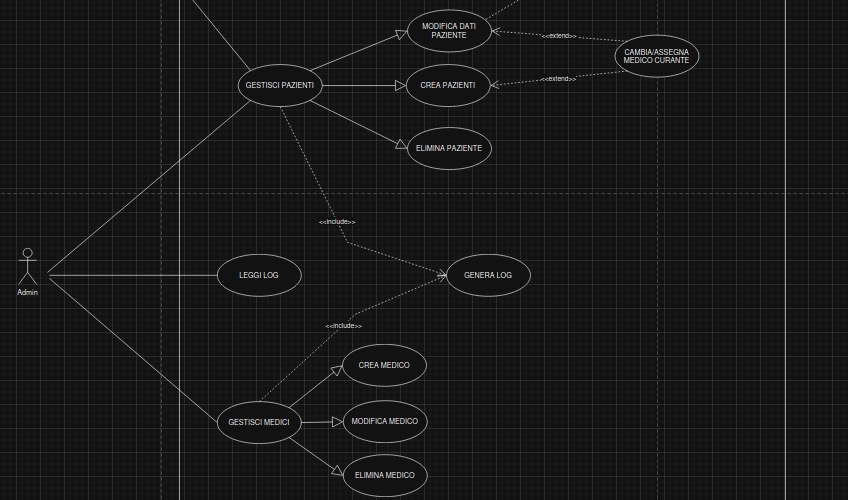
\includegraphics[width=\textwidth, height=\textheight, keepaspectratio]
    {img_relazione/Use_case_admin.png}
\end{figure}







\end{document}